\section{系统概览}
\subsection{系统架构}
为提高并发,提升应用性能,本案采用分布式系统设计,如图\ref{org} 所示,

\begin{figure}[htbp!]
    \centering
    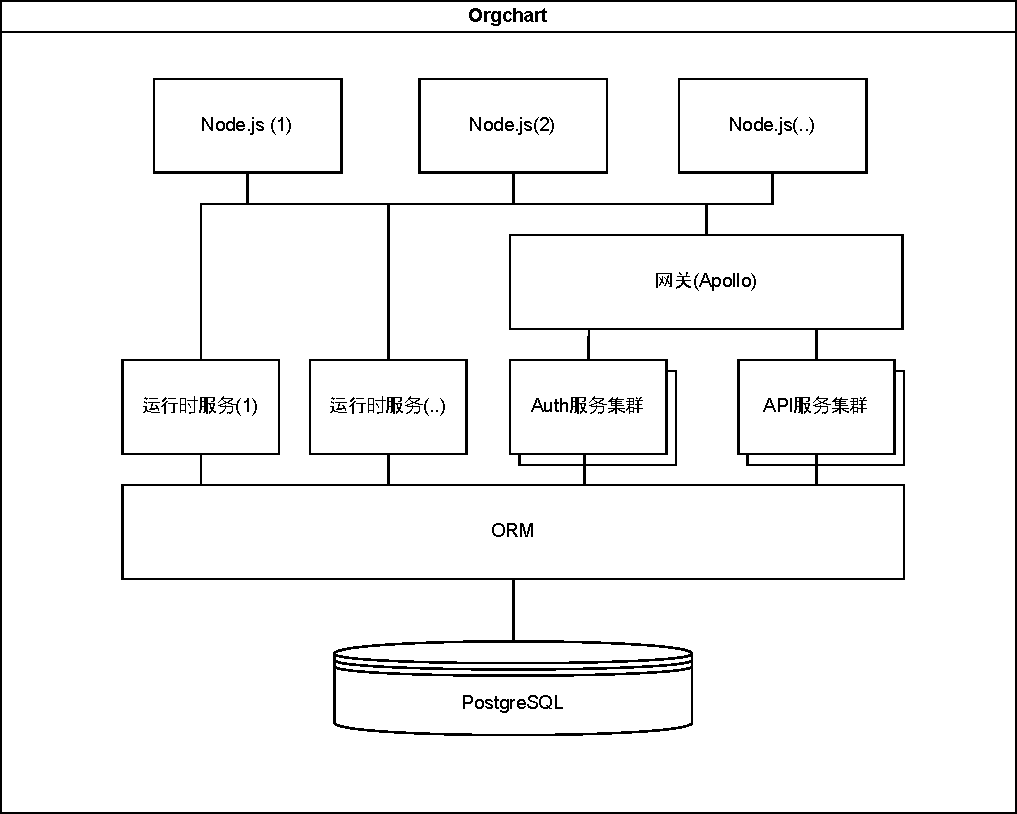
\includegraphics[width=0.95\textwidth]{figures/pdf/org.pdf}
    \caption{\label{org}系统架构组织图}
\end{figure}

本案符合非典型的web应用层次结构,分为表现层,接入层,业务逻辑层,数据访问层,
其中数据访问层采用名为 diesel 的 Rust crate 作为 ORM。
业务逻辑层分为Auth、API、Runtime等数个服务,每个服务都是独立的应用,可以横向扩展组成集群。
接入层使用 Apollo 作为 GraphQL 的网关,向外暴露所有的服务接口,还可以进行流量控制,但为了
支持运行时(Runtime)服务的“热插拔”,运行时服务并不会使用网关。
表现层使用 Node.js 作为 Web 的运行时,使用 React 作为 GUI 框架。
表现层和接入层、业务逻辑层使用 GraphQL 实现 Schema,使用 HTTP 和 WebSocket 协议通信,
并使用 actix-web 作为web服务端。

\subsection{生命周期与任务调度}
一个典型的实例生命周期由以下几部分组成
\begin{enumerate}
    \item 创建车站
    \item 创建实例
    \item 初始化实例
    \item 访问实例
    \item 结束实例
\end{enumerate}

其中,创建车站就需要用到后文提到的车站描述文件,车站被创建后将存入数据库中。创建好车站后,就可以创建
这个车站的实例。本案支持预约或称定时开始的实例,在开始之前若用户尝试在executor
初始化一个实例,就会报错。在GUI上,在开始时间之前,不渲染开始按钮,和后端的时间约束形成两层约束。
实例创建后同样也会被记录在数据库中,当时间到后用户就可以在创建实例时指定的executor上
初始化实例 -- executor从数据库中读入instance,并运行。
实例初始化后用户就可以在该实例中进行进路车辆的各种操作。
最后实例会被结束。

